\documentclass[12pt,a4paper]{article}

\usepackage{tocloft}
\renewcommand{\cftsecleader}{\cftdotfill{\cftdotsep}}
\cftsetindents{section}{0em}{4em}
\cftsetindents{subsection}{1em}{4em}
\usepackage{xcolor}
\usepackage{verbatim}
\usepackage{listings}
\usepackage{vntex}
\usepackage{a4wide,amssymb,epsfig,latexsym,array,hhline,fancyhdr}
\usepackage{enumitem}
\usepackage{MnSymbol,wasysym}
\usepackage{tikzsymbols}
\usepackage{textcomp}
\usepackage{parskip}
\usepackage[normalem]{ulem}
\usepackage{graphicx}
\usepackage[makeroom]{cancel}
\usepackage{amsmath}
\usepackage{amsthm}
\usepackage{multicol,longtable,amscd}
\usepackage{diagbox}
\usepackage{booktabs}
\usepackage{alltt}
\usepackage[framemethod=tikz]{mdframed}
\usepackage{caption,subcaption}
\usepackage{minted}
\usepackage{lastpage}
\usepackage[lined,boxed,commentsnumbered]{algorithm2e}
\usepackage{color}
\usepackage{array}
\usepackage{tabularx}
\usepackage{multirow}
\usepackage{rotating}
\usepackage{graphics}
\usepackage{geometry}
\usepackage{setspace}
\usepackage{tcolorbox}
\usepackage{float}
\usepackage{changepage}

\renewcommand\thepart{\Alph{part}}
\renewcommand\thesection{\Roman{section}}
\renewcommand\thesubsection{\arabic{subsection}}

\usepackage{titlesec}

%============================
% Cỡ chữ tiêu đề
%============================

\titleformat{\section}
{\fontsize{18pt}{22pt}\bfseries}
{\thesection}
{1em}
{}

\titleformat{\subsection}
{\fontsize{16pt}{20pt}\bfseries}
{\thesubsection}
{1em}
{}

\titleformat{\subsubsection}
{\fontsize{14pt}{18pt}\bfseries}
{\thesubsubsection}
{1em}
{}

\usepackage{tikz}
\usetikzlibrary{arrows,snakes,backgrounds}

% Hyperref nên để gần cuối
\usepackage{hyperref}
\hypersetup{
    colorlinks=true,
    linkcolor=black
}

% Nội dung
\setlength{\parindent}{0.4cm}
\setstretch{1.3}

\makeatletter
\renewcommand\tableofcontents{%
  \section*{\centering\contentsname
    \@mkboth{%
      \MakeUppercase\contentsname}{\MakeUppercase\contentsname}}%
  \@starttoc{toc}%
}

\makeatother

\setlength{\headheight}{40pt}
\pagestyle{fancy}
\fancyhead{} % clear all header fields
\fancyhead[L]{
 \begin{tabular}{rl}
    \begin{picture}(25,15)(0,0)
    \put(0,-8){
\includegraphics[width=8mm, height=8mm]{include/image/hcmut.png}}
   \end{picture}&
	\begin{tabular}{l}
		\textbf{\bf \ttfamily Trường đại học Bách Khoa thành phố Hồ Chí Minh}\\
		\textbf{\bf \ttfamily Khoa Khoa học và kĩ thuật máy tính}
	\end{tabular} 	
 \end{tabular}
}
\fancyhead[R]{
	\begin{tabular}{l}
		\tiny \bf \\
		\tiny \bf 
	\end{tabular}  }
\fancyfoot{} % clear all footer fields
\renewcommand{\headrulewidth}{0.3pt}
\renewcommand{\footrulewidth}{0.3pt}
\fancyfoot[R]{\scriptsize \ttfamily \textbf{\textcolor{red}{Trang}} {\textbf{\textcolor{red}{\thepage}}}/\pageref{LastPage}}
\renewcommand{\headrulewidth}{0.3pt}
\renewcommand{\footrulewidth}{0.3pt}
\setcounter{secnumdepth}{4}
\setcounter{tocdepth}{3}
\makeatletter
\newcounter {subsubsubsection}[subsubsection]
\renewcommand\thesubsubsubsection{\thesubsubsection .\@alph\c@subsubsubsection}
\newcommand\subsubsubsection{\@startsection{subsubsubsection}{4}{\z@}%
                                     {-3.25ex\@plus -1ex \@minus -.2ex}%
                                     {1.5ex \@plus .2ex}%
                                     {\normalfont\normalsize\bfseries}}
\newcommand*\l@subsubsubsection{\@dottedtocline{3}{10.0em}{4.1em}}
\newcommand*{\subsubsubsectionmark}[1]{}
\makeatother
\makeatletter
\providecommand*{\toclevel@subsubsubsection}{4}
\makeatother



\setlength{\parindent}{0pt}
\usepackage{graphicx} 
\usepackage{xcolor}
\usepackage{tikz} 
\usepackage{scrextend}
\changefontsizes{14pt}
\usetikzlibrary{calc}

\newmdenv[linecolor=black,skipabove=\topsep,skipbelow=\topsep,
leftmargin=-5pt,rightmargin=-5pt,
innerleftmargin=5pt,innerrightmargin=5pt]{mybox}
\newcommand{\safeincludegraphics}[2][]{%
    \IfFileExists{#2}{%
        \includegraphics[#1]{#2}%
    }{%
        \fbox{\parbox{0.9\textwidth}{\centering Hình minh họa chưa được bổ sung: \texttt{\detokenize{#2}}}}%
    }%
}
\def\thesislayout{	% A4: 210 × 297
	\geometry{
		a4paper,
		total={160mm,240mm},  % fix over page
		left=30mm,
		top=30mm,
	}
}
\lstset{
    language=R,
    basicstyle=\ttfamily\small,
    keywordstyle=\color{black}\ttfamily,
    stringstyle=\color{black}\ttfamily,
    commentstyle=\color{green}\ttfamily,
    morecomment=[l][\color{magenta}]{\#},
    numbers=left,
    numberstyle=\tiny\color{gray},
    stepnumber=1,
    numbersep=10pt,
    backgroundcolor=\color{white},
    tabsize=4,
    showspaces=false,
    showstringspaces=false,
    breaklines=true
}
\thesislayout
\begin{document}

\begin{titlepage}
\begin{tikzpicture}[remember picture,overlay,inner sep=0,outer sep=0]
     \draw[blue!70!black,line width=4pt] ([xshift=-1.5cm,yshift=-2cm]current page.north east) coordinate (A)--([xshift=1.5cm,yshift=-2cm]current page.north west) coordinate(B)--([xshift=1.5cm,yshift=2cm]current page.south west) coordinate (C)--([xshift=-1.5cm,yshift=2cm]current page.south east) coordinate(D)--cycle;

     \draw ([yshift=0.5cm,xshift=-0.5cm]A)-- ([yshift=0.5cm,xshift=0.5cm]B)--
     ([yshift=-0.5cm,xshift=0.5cm]B) --([yshift=-0.5cm,xshift=-0.5cm]B)--([yshift=0.5cm,xshift=-0.5cm]C)--([yshift=0.5cm,xshift=0.5cm]C)--([yshift=-0.5cm,xshift=0.5cm]C)-- ([yshift=-0.5cm,xshift=-0.5cm]D)--([yshift=0.5cm,xshift=-0.5cm]D)--([yshift=0.5cm,xshift=0.5cm]D)--([yshift=-0.5cm,xshift=0.5cm]A)--([yshift=-0.5cm,xshift=-0.5cm]A)--([yshift=0.5cm,xshift=-0.5cm]A);


     \draw ([yshift=-0.3cm,xshift=0.3cm]A)-- ([yshift=-0.3cm,xshift=-0.3cm]B)--
     ([yshift=0.3cm,xshift=-0.3cm]B) --([yshift=0.3cm,xshift=0.3cm]B)--([yshift=-0.3cm,xshift=0.3cm]C)--([yshift=-0.3cm,xshift=-0.3cm]C)--([yshift=0.3cm,xshift=-0.3cm]C)-- ([yshift=0.3cm,xshift=0.3cm]D)--([yshift=-0.3cm,xshift=0.3cm]D)--([yshift=-0.3cm,xshift=-0.3cm]D)--([yshift=0.3cm,xshift=-0.3cm]A)--([yshift=0.3cm,xshift=0.3cm]A)--([yshift=-0.3cm,xshift=0.3cm]A);

   \end{tikzpicture}
\begin{center}
    \vspace{-2cm}
    \fontsize{16pt}{17pt}\selectfont 
    \textbf{\\ĐẠI HỌC QUỐC GIA TP. HỒ CHÍ MINH}
    \textbf{\\TRƯỜNG ĐẠI HỌC BÁCH KHOA}
    

\end{center}
 \vspace{10pt}
 \begin{center}
     
\includegraphics[scale=1]{include/image/hcmut.png}
 \end{center}

\begin{center}
    \fontsize{14pt}{0pt}\selectfont \textbf{BÁO CÁO}\\
    \textbf{ĐỒ ÁN THỰC TẬP NGOÀI TRƯỜNG }\\
    \textbf{HỌC KỲ 3 NĂM HỌC 2025-2026}\\
    \textbf{NGÀNH: KỸ THUẬT MÁY TÍNH}\\
    \textbf{CHƯƠNG TRÌNH ĐÀO TẠO: CHÍNH QUY}
\vspace{0.5cm}

\fontsize{14pt}{18pt} \selectfont \textbf{ĐỀ TÀI:\\ PHÁT TRIỂN HỆ THỐNG IOT HỖ TRỢ GIÁM SÁT, QUẢN LÍ VÀ BẢO TRÌ MÁY LỌC NƯỚC THEO THỜI GIAN THỰC} \\
\vspace{0.5cm} \textbf{ĐƠN VỊ/DOANH NGHIỆP THỰC TẬP: TRUNG TÂM DỊCH VỤ KHÁCH HÀNG (HSC) - CÔNG TY CỔ PHẦN DỊCH VỤ CÔNG NGHỆ THÔNG TIN HPT}

\end{center}
\vspace{2pt}
\centering
 \textbf{GIẢNG VIÊN HƯỚNG DẪN: NGUYỄN THÀNH LỘC
 \\
   }

\fontsize{12pt}{25pt}\selectfont
{\textbf{SINH VIÊN THỰC HIỆN: HOÀNG ANH DUY}\\
\textbf{MÃ SỐ SINH VIÊN: 2310458 }}
\end{titlepage}


\newpage
\footnotesize
\tableofcontents
\thispagestyle{empty}
\addtocontents{toc}{\protect\thispagestyle{empty}}

\large
\newpage
\footnotesize
\phantomsection
    \vspace{-2cm}
\newpage
\pagenumbering{arabic}

\section{GIỚI THIỆU}

\subsection{Giới thiệu về Công ty Cổ phần Dịch vụ Công nghệ Tin học HPT}

Công ty Cổ phần Dịch vụ Công nghệ Tin học HPT (HPT) là một trong những doanh nghiệp công nghệ thông tin hàng đầu tại Việt Nam với hơn 30 năm hình thành và phát triển. HPT hoạt động trong nhiều lĩnh vực như tư vấn và triển khai giải pháp công nghệ thông tin, tích hợp hệ thống, phát triển phần mềm, cung cấp dịch vụ chuyển đổi số, điện toán đám mây, an toàn thông tin, quản trị hạ tầng CNTT, đào tạo và cung ứng nguồn nhân lực công nghệ thông tin.

Trong suốt quá trình phát triển, HPT đã xây dựng được đội ngũ chuyên gia và kỹ sư giàu kinh nghiệm, không ngừng nghiên cứu và tiếp cận các công nghệ hiện đại như điện toán đám mây (Cloud Computing), trí tuệ nhân tạo (Artificial Intelligence), dữ liệu lớn (Big Data), Internet vạn vật (IoT) và các giải pháp chuyển đổi số cho doanh nghiệp. Với năng lực chuyên môn cao cùng kinh nghiệm triển khai nhiều dự án quy mô lớn, HPT đã trở thành đối tác tin cậy của nhiều tổ chức, doanh nghiệp và cơ quan trọng yếu tại Việt Nam.

Bên cạnh năng lực công nghệ, HPT còn chú trọng xây dựng môi trường làm việc chuyên nghiệp, đề cao giá trị văn hóa doanh nghiệp với phương châm ``Nhân bản -- Hài hòa'', tạo điều kiện cho nhân viên phát triển chuyên môn và đóng góp vào sự phát triển bền vững của doanh nghiệp. Hệ thống quy trình quản lý dự án, quản lý chất lượng và phát triển sản phẩm được xây dựng theo các chuẩn quốc tế nhằm đảm bảo chất lượng dịch vụ và nâng cao hiệu quả triển khai dự án.

\subsection{Giới thiệu nội dung thực tập}

Trong thời gian thực tập tại HPT, sinh viên được tham gia tìm hiểu môi trường làm việc thực tế của doanh nghiệp, quy trình quản lý dự án theo chuẩn CMMI, mô hình phát triển Agile Scrum cũng như các hoạt động quản lý chất lượng, quản lý rủi ro và phối hợp với khách hàng trong quá trình triển khai dự án.

Bên cạnh việc tìm hiểu các quy trình quản lý dự án, sinh viên còn được tiếp cận với dự án thực tế trong lĩnh vực Internet of Things (IoT). Dự án hướng đến xây dựng hệ thống giám sát, quản lý và bảo trì máy lọc nước từ xa theo thời gian thực. Thông qua dự án này, sinh viên có cơ hội tìm hiểu kiến trúc hệ thống IoT, quy trình thu thập và xử lý dữ liệu từ thiết bị nhúng, cơ chế truyền thông giữa thiết bị và máy chủ, cũng như các công nghệ được sử dụng trong quá trình phát triển sản phẩm tại doanh nghiệp.

Đợt thực tập là cơ hội để vận dụng kiến thức đã học vào môi trường thực tế, đồng thời nâng cao kỹ năng chuyên môn, kỹ năng làm việc nhóm và hiểu rõ hơn về quy trình phát triển và triển khai các dự án công nghệ thông tin trong doanh nghiệp.
\section{NỘI DUNG THỰC TẬP}

\subsection{Thông tin đề tài thực tập}

\textbf{Tên đề tài:} Phát triển hệ thống IoT hỗ trợ giám sát, quản lý và bảo trì máy lọc nước theo thời gian thực.

\textbf{Ngôn ngữ lập trình sử dụng:}
\begin{itemize}
    \item C/C++
    \item C\#
    \item JavaScript
    \item SQL
\end{itemize}

\textbf{Framework và công nghệ sử dụng:}
\begin{itemize}
    \item Arduino Framework
    \item MQTTnet
    \item ASP.NET Core MVC
    \item MQTT Broker
    \item Hệ quản trị cơ sở dữ liệu SQL
\end{itemize}

\subsection{Mục tiêu thực tập}

Mục tiêu của đợt thực tập là tìm hiểu quy trình phát triển hệ thống IoT trong môi trường doanh nghiệp, nghiên cứu kiến trúc hệ thống máy lọc nước thông minh và tham gia xây dựng các thành phần của hệ thống từ thiết bị phần cứng đến nền tảng quản lý tập trung. Bên cạnh đó, sinh viên được tiếp cận với các công nghệ Web Backend, giao thức truyền thông MQTT và quy trình phát triển phần mềm thực tế.

\subsection{Nội dung công việc thực hiện}

Trong suốt thời gian thực tập, các công việc được thực hiện theo từng giai đoạn như sau:

\begin{table}[htbp]
    \centering
    \begin{tabularx}{\textwidth}{|>{\centering\arraybackslash}p{2cm}|X|}
        \hline
        \textbf{Tuần} & \textbf{Nội dung công việc} \\
        \hline
        1 & Tìm hiểu về công ty, môi trường làm việc, quy trình phát triển sản phẩm và định hướng thực tập. \\
        \hline
        2 & Nghiên cứu hệ thống hiện tại của dự án, tìm hiểu kiến trúc giải pháp, quy trình nghiệp vụ và mô hình IoT đang được áp dụng. \\
        \hline
        3 & Làm quen với hệ thống Web Backend, khảo sát kiến trúc dữ liệu và luồng xử lý dữ liệu trong hệ thống. \\
        \hline
        4 & Khảo sát phần cứng máy lọc nước, nghiên cứu sơ đồ điều khiển, các cảm biến được sử dụng và đánh giá khả năng tích hợp IoT vào thiết bị. \\
        \hline
        5 & Tìm hiểu giao thức MQTT, thực hiện kết nối thiết bị với MQTT Broker và xây dựng cơ chế truyền dữ liệu từ thiết bị lên hệ thống quản lý. \\
        \hline
        6 & Tham gia phát triển các chức năng thu thập, xử lý và lưu trữ dữ liệu từ máy lọc nước; xây dựng giao diện Dashboard hỗ trợ giám sát thiết bị theo thời gian thực. \\
        \hline
        7 & Kiểm thử hệ thống, đánh giá kết quả hoạt động, tối ưu và hoàn thiện các chức năng được giao. \\
        \hline
        8 & Tổng hợp kết quả thực hiện, hoàn thiện tài liệu kỹ thuật và báo cáo thực tập. \\
        \hline
    \end{tabularx}
\end{table}
\subsection{Tuần 1}

\subsubsection{Nội dung công việc: Tìm hiểu về công ty, môi trường làm việc, quy trình phát triển sản phẩm và định hướng thực tập.}
\textbf{Hoạt động:}
\begin{itemize}
    \item Tham gia chương trình định hướng thực tập, tìm hiểu về lịch sử hình thành, cơ cấu tổ chức và lĩnh vực hoạt động của công ty.
    
    \item Tìm hiểu môi trường làm việc, quy định nội bộ, quy trình làm việc và văn hóa doanh nghiệp.
    
    \item Nghiên cứu tổng quan về quản lý dự án trong lĩnh vực công nghệ thông tin.
    
    \item Tìm hiểu mô hình quản lý dự án theo chuẩn CMMI được áp dụng tại công ty.
    
    \item Nghiên cứu các giai đoạn trong vòng đời quản lý dự án bao gồm: khởi động, xác định yêu cầu, lập giải pháp, xây dựng, triển khai và kết thúc dự án.
    
    \item Tìm hiểu quy trình hoạch định dự án, xác định phạm vi công việc, lập kế hoạch nguồn lực và tiến độ thực hiện.
    
    \item Tìm hiểu cơ cấu tổ chức nhân sự trong dự án và vai trò của các thành viên tham gia dự án.
    
    \item Nghiên cứu mô hình làm việc Agile Scrum và cách tổ chức đội dự án theo Scrum Team.
    
    \item Tìm hiểu vai trò của Product Owner, Scrum Master và Development Team trong quá trình phát triển sản phẩm.
    
    \item Tìm hiểu các hoạt động quản lý yêu cầu khách hàng và quy trình phối hợp giữa khách hàng với đội dự án.
    
    \item Nghiên cứu quy trình quản lý thay đổi yêu cầu trong quá trình thực hiện dự án.
    
    \item Tìm hiểu quy trình quản lý rủi ro và các biện pháp giảm thiểu rủi ro trong dự án phần mềm.
    
    \item Tìm hiểu các hoạt động đảm bảo chất lượng (Quality Assurance) và kiểm thử phần mềm.
    
    \item Tìm hiểu quy trình triển khai hệ thống, hỗ trợ khách hàng, nghiệm thu và bàn giao sản phẩm.
    
    \item Tìm hiểu chính sách bảo hành, bảo trì và hỗ trợ sau triển khai của doanh nghiệp.
    
    \item Tìm hiểu tổng quan về dự án thực tập, nghiệp vụ của dự án và các công nghệ dự kiến được sử dụng trong quá trình thực hiện.
\end{itemize}
\subsubsection{Nội dung tìm hiểu và kiến thức thu nhận}

\paragraph{1. Tổng quan về quản lý dự án}

Quản lý dự án (Project Management) là quá trình áp dụng kiến thức, kỹ năng, công cụ và kỹ thuật nhằm lập kế hoạch, tổ chức, giám sát và kiểm soát các hoạt động của dự án để đạt được các mục tiêu đã đề ra. Trong lĩnh vực công nghệ thông tin, quản lý dự án đóng vai trò quan trọng trong việc đảm bảo sản phẩm được phát triển đúng phạm vi, đáp ứng yêu cầu khách hàng, hoàn thành đúng tiến độ và tối ưu chi phí thực hiện.

Một dự án phần mềm thường phải cân bằng giữa ba yếu tố chính gồm phạm vi công việc (Scope), thời gian thực hiện (Time) và chi phí (Cost). Bên cạnh đó, chất lượng sản phẩm (Quality) cũng là một yếu tố quan trọng quyết định sự thành công của dự án. Do đó, các doanh nghiệp thường xây dựng những quy trình quản lý chặt chẽ nhằm giảm thiểu rủi ro và nâng cao hiệu quả triển khai dự án.

\paragraph{2. Quy trình quản lý dự án theo chuẩn CMMI}

\begin{figure}[h]
    \centering
    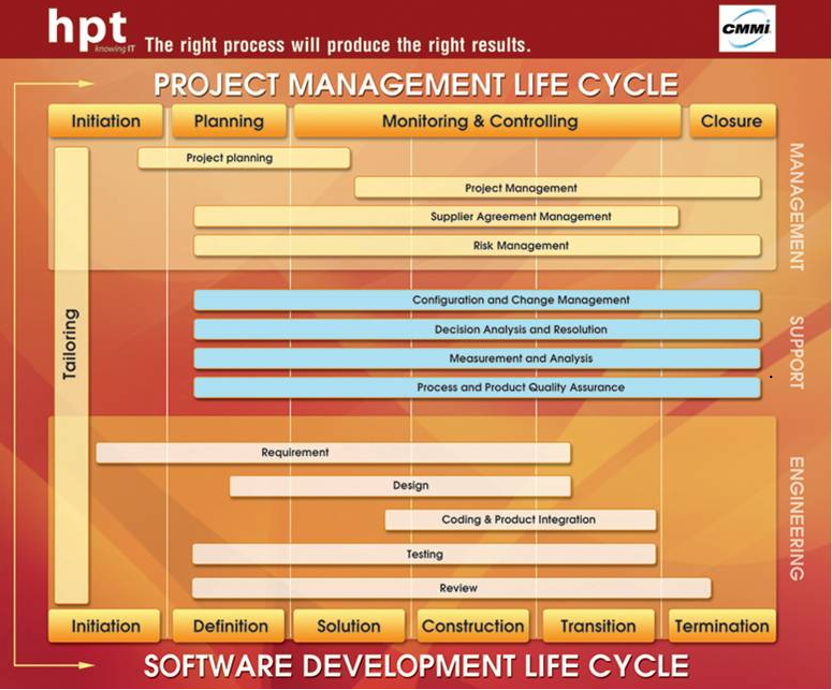
\includegraphics[width=0.8\textwidth]{include/image/cmmi.png}
    \caption{Quy trình CMMI cho phát triển phần mềm}
    \label{fig:cmmi}
\end{figure}

Qua quá trình tìm hiểu, công ty áp dụng mô hình CMMI (Capability Maturity Model Integration) trong quản lý và triển khai dự án phần mềm. Đây là một mô hình cải tiến quy trình được sử dụng rộng rãi trong ngành công nghệ thông tin nhằm chuẩn hóa hoạt động quản lý, nâng cao chất lượng sản phẩm và tăng khả năng thành công của dự án.

Theo mô hình này, dự án được chia thành nhiều giai đoạn với các mục tiêu, sản phẩm đầu ra và tiêu chí đánh giá cụ thể. Mỗi giai đoạn đều phải được xem xét, đánh giá và phê duyệt trước khi chuyển sang giai đoạn tiếp theo nhằm đảm bảo chất lượng của toàn bộ dự án.

\subparagraph{Giai đoạn khởi động}

Đây là giai đoạn đầu tiên của dự án, có nhiệm vụ xác định mục tiêu, phạm vi và tính khả thi của dự án. Các hoạt động chính bao gồm khảo sát nhu cầu khách hàng, xác định phạm vi công việc, ước lượng nguồn lực, xây dựng kế hoạch sơ bộ và ban hành quyết định khởi động dự án.

Kết quả của giai đoạn này là một kế hoạch tổng quan giúp các bên liên quan có được cái nhìn chung về mục tiêu và định hướng thực hiện dự án.

\subparagraph{Giai đoạn xác định yêu cầu}

Mục tiêu của giai đoạn này là thu thập, phân tích và làm rõ các yêu cầu từ khách hàng. Các yêu cầu được chuyển đổi thành các tài liệu đặc tả giúp đội phát triển hiểu rõ chức năng và đặc điểm của hệ thống cần xây dựng.

Trong quá trình này, các chuyên gia nghiệp vụ và phân tích hệ thống sẽ phối hợp với khách hàng để làm rõ các yêu cầu chức năng, yêu cầu phi chức năng, tiêu chí nghiệm thu và các ràng buộc của dự án. Đây là một trong những giai đoạn quan trọng nhất vì các sai sót trong việc xác định yêu cầu có thể ảnh hưởng đến toàn bộ quá trình phát triển sau này.

\subparagraph{Giai đoạn lập giải pháp}

Sau khi các yêu cầu được xác nhận, nhóm dự án tiến hành xây dựng các giải pháp kỹ thuật phù hợp. Công việc chính bao gồm thiết kế kiến trúc hệ thống, xác định các thành phần phần mềm, cơ sở dữ liệu, giao diện và các cơ chế tích hợp giữa các hệ thống.

Giai đoạn này giúp chuyển đổi các yêu cầu nghiệp vụ thành các giải pháp kỹ thuật cụ thể, đồng thời đánh giá tính khả thi của hệ thống trước khi tiến hành phát triển.

\subparagraph{Giai đoạn xây dựng}

Đây là giai đoạn hiện thực hóa các thiết kế thành sản phẩm phần mềm hoàn chỉnh. Các lập trình viên tiến hành phát triển các chức năng theo tài liệu thiết kế, đồng thời thực hiện kiểm thử đơn vị và kiểm thử tích hợp nhằm phát hiện sớm các lỗi phát sinh.

Bên cạnh hoạt động lập trình, các hoạt động kiểm thử và kiểm soát chất lượng cũng được thực hiện liên tục nhằm đảm bảo sản phẩm đáp ứng các tiêu chuẩn kỹ thuật đã đề ra.

\subparagraph{Giai đoạn triển khai}

Sau khi sản phẩm hoàn thiện và đạt yêu cầu chất lượng, hệ thống được triển khai lên môi trường thực tế. Các hoạt động chính bao gồm cài đặt hệ thống, cấu hình môi trường vận hành, hỗ trợ kiểm thử nghiệm thu và đào tạo người sử dụng.

Mục tiêu của giai đoạn này là đảm bảo khách hàng có thể sử dụng hệ thống một cách hiệu quả và ổn định trong môi trường thực tế.

\subparagraph{Giai đoạn kết thúc}

Giai đoạn kết thúc được thực hiện sau khi khách hàng hoàn thành việc nghiệm thu sản phẩm. Các tài liệu dự án, mã nguồn và các sản phẩm liên quan được tổng hợp và bàn giao cho bộ phận quản lý hoặc khách hàng theo quy định.

Ngoài ra, các bài học kinh nghiệm, phản hồi từ khách hàng và các chỉ số chất lượng cũng được thu thập nhằm phục vụ cho việc cải tiến quy trình và triển khai các dự án trong tương lai.

\paragraph{3. Hoạch định dự án}

Hoạch định dự án là hoạt động quan trọng nhằm xác định phương án triển khai dự án trước khi bắt đầu thực hiện. Nội dung hoạch định bao gồm xác định phạm vi công việc, phân chia nhiệm vụ, ước lượng nguồn lực, xây dựng kế hoạch tiến độ và xác định các mốc quan trọng của dự án.

Thông qua hoạt động hoạch định, nhóm dự án có thể dự đoán trước các khó khăn có thể phát sinh, phân bổ nguồn lực hợp lý và xây dựng các phương án ứng phó với rủi ro. Một kế hoạch tốt sẽ giúp tăng khả năng hoàn thành dự án đúng tiến độ và đáp ứng các mục tiêu đã đề ra.

Trong thực tế, kế hoạch dự án thường được cập nhật định kỳ để phản ánh các thay đổi về yêu cầu, nguồn lực hoặc các điều kiện triển khai thực tế.

Việc phân công vai trò rõ ràng giúp giảm thiểu sự chồng chéo trách nhiệm, nâng cao hiệu quả phối hợp và đảm bảo dự án được triển khai một cách có hệ thống.


\paragraph{5. Mô hình Scrum}

Bên cạnh quy trình quản lý dự án theo chuẩn CMMI, doanh nghiệp còn áp dụng phương pháp Agile Scrum trong quá trình phát triển sản phẩm nhằm nâng cao khả năng thích ứng với sự thay đổi của yêu cầu khách hàng và tăng hiệu quả phối hợp giữa các thành viên trong dự án.

Scrum là một framework thuộc Agile, được xây dựng dựa trên nguyên tắc phát triển lặp và tăng trưởng (Iterative and Incremental Development). Thay vì xây dựng toàn bộ hệ thống trong một chu kỳ dài, Scrum chia dự án thành nhiều chu kỳ ngắn gọi là Sprint. Sau mỗi Sprint, nhóm phát triển sẽ tạo ra một phần sản phẩm có thể kiểm thử và đánh giá được.

Mô hình Scrum tập trung vào tính minh bạch, khả năng thích nghi và cải tiến liên tục, giúp nhóm phát triển nhanh chóng phát hiện vấn đề và điều chỉnh kế hoạch khi cần thiết.

\begin{figure}[h]
    \centering
    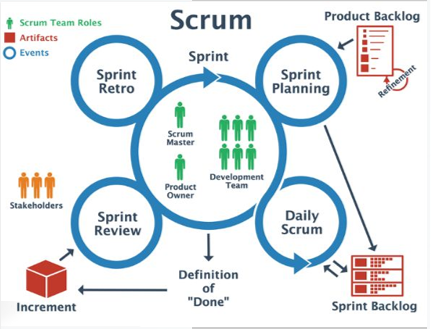
\includegraphics[width=0.8\textwidth]{include/image/scrum.png}
    \label{fig:scrum}
\end{figure}

\subparagraph{Product Owner}

Product Owner là người đại diện cho khách hàng hoặc các bên liên quan của dự án. Vai trò chính của Product Owner là xác định giá trị kinh doanh của sản phẩm và đảm bảo nhóm phát triển luôn tập trung vào những chức năng mang lại giá trị cao nhất.

Các nhiệm vụ chính của Product Owner bao gồm:

\begin{itemize}
\item Thu thập và làm rõ yêu cầu từ khách hàng.
\item Xây dựng và quản lý danh sách yêu cầu của sản phẩm.
\item Xác định mức độ ưu tiên của các chức năng.
\item Đưa ra quyết định liên quan đến phạm vi sản phẩm.
\item Tham gia đánh giá kết quả sau mỗi Sprint.
\end{itemize}

Product Owner đóng vai trò cầu nối giữa khách hàng và đội phát triển, đảm bảo sản phẩm cuối cùng đáp ứng đúng nhu cầu nghiệp vụ.

\subparagraph{Scrum Master}

Scrum Master là người chịu trách nhiệm đảm bảo nhóm làm việc đúng theo các nguyên tắc và quy trình Scrum.

Vai trò của Scrum Master không phải là quản lý trực tiếp các thành viên mà là hỗ trợ nhóm làm việc hiệu quả hơn bằng cách:

\begin{itemize}
\item Hướng dẫn nhóm áp dụng Scrum.
\item Tổ chức các cuộc họp Scrum.
\item Loại bỏ các trở ngại ảnh hưởng đến tiến độ công việc.
\item Hỗ trợ giao tiếp giữa các thành viên và các bên liên quan.
\item Thúc đẩy quá trình cải tiến liên tục trong nhóm.
\end{itemize}

Thông qua vai trò này, Scrum Master giúp nhóm duy trì năng suất và đảm bảo quá trình phát triển diễn ra ổn định.

\subparagraph{Development Team}

Development Team là nhóm chịu trách nhiệm trực tiếp xây dựng sản phẩm.

Tùy thuộc vào quy mô dự án, nhóm có thể bao gồm:

\begin{itemize}
\item Software Developer.
\item Frontend Developer.
\item Backend Developer.
\item Embedded Engineer.
\item Tester.
\item QA Engineer.
\item DevOps Engineer.
\end{itemize}

Đặc điểm của Development Team là tính tự quản (Self-organizing), nghĩa là các thành viên chủ động phân chia công việc, phối hợp với nhau để hoàn thành mục tiêu của Sprint thay vì phụ thuộc hoàn toàn vào cấp quản lý.

Mọi thành viên đều có trách nhiệm đóng góp vào việc hoàn thành sản phẩm và đảm bảo chất lượng của các chức năng được phát triển.

\subparagraph{Sprint}

Sprint là đơn vị thời gian cơ bản trong Scrum, thường kéo dài từ một đến bốn tuần.

Trong mỗi Sprint, nhóm phát triển sẽ thực hiện một tập hợp các công việc đã được lựa chọn trước đó và cố gắng hoàn thành chúng trong khoảng thời gian cố định.

Mỗi Sprint thường bao gồm các hoạt động:

\begin{itemize}
\item Sprint Planning.
\item Development.
\item Daily Scrum.
\item Sprint Review.
\item Sprint Retrospective.
\end{itemize}

Kết thúc Sprint, nhóm sẽ tạo ra một phiên bản sản phẩm có thể trình diễn hoặc triển khai thử nghiệm. Điều này giúp khách hàng đánh giá kết quả sớm và đưa ra phản hồi kịp thời.

\subparagraph{Product Backlog}

Product Backlog là danh sách toàn bộ các yêu cầu, chức năng, cải tiến hoặc sửa lỗi của sản phẩm.

Danh sách này được quản lý bởi Product Owner và luôn được cập nhật trong suốt vòng đời dự án.

Mỗi mục trong Product Backlog thường bao gồm:

\begin{itemize}
\item Mô tả yêu cầu.
\item Mức độ ưu tiên.
\item Giá trị nghiệp vụ.
\item Ước lượng khối lượng công việc.
\end{itemize}

Product Backlog đóng vai trò như nguồn công việc trung tâm của toàn bộ dự án và là cơ sở để lập kế hoạch cho các Sprint tiếp theo.

\subparagraph{Sprint Backlog}

Sprint Backlog là tập hợp các công việc được lựa chọn từ Product Backlog để thực hiện trong một Sprint cụ thể.

Trong cuộc họp Sprint Planning, Development Team cùng Product Owner sẽ lựa chọn các hạng mục phù hợp với năng lực thực hiện của nhóm trong khoảng thời gian Sprint.

Sprint Backlog giúp:

\begin{itemize}
\item Xác định rõ mục tiêu của Sprint.
\item Theo dõi tiến độ thực hiện công việc.
\item Đánh giá năng suất của nhóm phát triển.
\item Hỗ trợ quản lý và phân công công việc.
\end{itemize}

Trong quá trình thực hiện Sprint, Sprint Backlog có thể được cập nhật để phản ánh trạng thái thực tế của các công việc đang triển khai.

Thông qua mô hình Scrum, doanh nghiệp có thể quản lý công việc linh hoạt hơn, tăng khả năng phản hồi trước các thay đổi từ khách hàng và nâng cao hiệu quả phối hợp giữa các thành viên trong dự án.


\paragraph{6. Quy trình phối hợp với khách hàng}

Khách hàng là một trong những bên liên quan quan trọng nhất của dự án. Việc phối hợp hiệu quả giữa đội dự án và khách hàng giúp đảm bảo sản phẩm được phát triển đúng với nhu cầu thực tế và hạn chế các sai lệch trong quá trình triển khai.

Quy trình phối hợp thường bắt đầu từ giai đoạn khảo sát và thu thập yêu cầu. Trong giai đoạn này, các buổi họp trao đổi được tổ chức nhằm làm rõ nghiệp vụ, xác định các yêu cầu chức năng và phi chức năng của hệ thống. Các yêu cầu sau khi được phân tích sẽ được xác nhận lại với khách hàng để đảm bảo sự thống nhất giữa hai bên.

Trong quá trình thực hiện dự án, đội dự án thường xuyên báo cáo tiến độ, trình bày các kết quả đạt được và tiếp nhận phản hồi từ khách hàng. Các cuộc họp định kỳ giúp theo dõi tình trạng dự án, xử lý các vấn đề phát sinh và cập nhật các thay đổi cần thiết.

Đến giai đoạn nghiệm thu, khách hàng tham gia đánh giá sản phẩm dựa trên các tiêu chí đã được thống nhất từ trước. Kết quả nghiệm thu là cơ sở để thực hiện bàn giao và đưa hệ thống vào vận hành chính thức.

\paragraph{7. Quản lý thay đổi}

Trong thực tế triển khai dự án, các yêu cầu thay đổi là điều khó tránh khỏi do sự thay đổi của nhu cầu nghiệp vụ, quy trình vận hành hoặc các yếu tố khách quan khác. Vì vậy, việc quản lý thay đổi đóng vai trò quan trọng nhằm kiểm soát tác động của các thay đổi đến phạm vi, tiến độ, chi phí và chất lượng dự án.

Quy trình quản lý thay đổi thường bao gồm các bước tiếp nhận yêu cầu thay đổi, phân tích tác động, đánh giá tính khả thi, phê duyệt và triển khai thực hiện. Mọi thay đổi đều cần được ghi nhận và đánh giá trước khi đưa vào kế hoạch thực hiện nhằm tránh phát sinh các rủi ro không mong muốn.

Việc phân tích tác động giúp xác định mức độ ảnh hưởng của thay đổi đối với hệ thống hiện tại, nguồn lực dự án và các hạng mục công việc đang thực hiện. Sau khi được phê duyệt, các thay đổi sẽ được cập nhật vào kế hoạch dự án và thông báo đến các bên liên quan.

Thông qua quy trình quản lý thay đổi, doanh nghiệp có thể duy trì sự linh hoạt trong phát triển sản phẩm đồng thời vẫn đảm bảo khả năng kiểm soát dự án.

\paragraph{8. Quản lý rủi ro}

Quản lý rủi ro là hoạt động nhằm nhận diện, đánh giá và xây dựng các biện pháp ứng phó đối với những sự kiện có khả năng ảnh hưởng tiêu cực đến dự án.

Các rủi ro trong dự án công nghệ thông tin có thể đến từ nhiều nguồn khác nhau như thay đổi yêu cầu, thiếu hụt nguồn lực, sai sót kỹ thuật, chậm tiến độ, sự cố hạ tầng hoặc các yếu tố liên quan đến khách hàng.

Quy trình quản lý rủi ro thường bao gồm bốn bước chính:

\begin{enumerate}
    \item Nhận diện rủi ro.
    \item Phân tích mức độ ảnh hưởng và xác suất xảy ra.
    \item Xây dựng phương án giảm thiểu hoặc ứng phó.
    \item Theo dõi và cập nhật trạng thái rủi ro.
\end{enumerate}

Các rủi ro có mức độ ưu tiên cao cần được theo dõi thường xuyên và có kế hoạch xử lý cụ thể. Việc quản lý rủi ro chủ động giúp giảm thiểu tổn thất, hạn chế chậm tiến độ và nâng cao khả năng thành công của dự án.

\paragraph{9. Đảm bảo chất lượng}

Đảm bảo chất lượng (Quality Assurance - QA) là tập hợp các hoạt động nhằm bảo đảm sản phẩm và quy trình phát triển đáp ứng các tiêu chuẩn chất lượng đã đề ra.

Trong các dự án phần mềm, chất lượng không chỉ được đánh giá thông qua sản phẩm cuối cùng mà còn được kiểm soát trong toàn bộ vòng đời dự án. Các hoạt động đảm bảo chất lượng bao gồm rà soát tài liệu, kiểm tra việc tuân thủ quy trình, đánh giá kết quả kiểm thử và theo dõi các chỉ số chất lượng.

Bên cạnh QA, hoạt động kiểm soát chất lượng (Quality Control - QC) cũng được thực hiện nhằm phát hiện lỗi trong sản phẩm thông qua các hoạt động kiểm thử. Nếu QA tập trung vào việc phòng ngừa lỗi thì QC tập trung vào việc phát hiện và khắc phục lỗi trước khi sản phẩm được bàn giao cho khách hàng.

Việc kết hợp giữa QA và QC giúp nâng cao độ tin cậy của sản phẩm, giảm chi phí sửa lỗi và tăng mức độ hài lòng của khách hàng.

\paragraph{10. Hỗ trợ, triển khai và bàn giao}

Sau khi sản phẩm hoàn thành và vượt qua các vòng kiểm thử nội bộ, hệ thống sẽ được triển khai tại môi trường thực tế của khách hàng. Giai đoạn này bao gồm các hoạt động cài đặt, cấu hình, kiểm tra vận hành và đào tạo người sử dụng.

Để đảm bảo khách hàng có thể khai thác hiệu quả hệ thống, đội dự án chuẩn bị các tài liệu hướng dẫn sử dụng, tài liệu vận hành và các nội dung đào tạo liên quan. Các buổi hướng dẫn và chuyển giao kiến thức giúp người sử dụng nhanh chóng làm quen với hệ thống mới.

Sau khi hoàn tất triển khai, khách hàng tiến hành nghiệm thu dựa trên các tiêu chí đã được thống nhất trong giai đoạn xác định yêu cầu. Khi sản phẩm đáp ứng đầy đủ các điều kiện nghiệm thu, đội dự án thực hiện bàn giao hệ thống, tài liệu liên quan và các sản phẩm của dự án cho khách hàng.

Ngoài ra, doanh nghiệp còn cung cấp các dịch vụ hỗ trợ sau triển khai như xử lý sự cố, bảo hành, bảo trì và nâng cấp hệ thống nhằm đảm bảo hệ thống vận hành ổn định trong suốt quá trình sử dụng.

\subsubsection{Tổng kết tuần 1}
\subsection{Tuần 2: Nghiên cứu hồ sơ đề xuất kỹ thuật và mô hình tổng thể}

\subsubsection{Nội dung công việc tuần 2}
Trong tuần thứ hai, em tập trung nghiên cứu hồ sơ đề xuất kỹ thuật để nắm được bài toán của dự án, cách tổ chức hệ thống ở mức tổng quan và phạm vi kiến thức cần chuẩn bị cho các tuần tiếp theo.

\begin{enumerate}
    \item Nghiên cứu hồ sơ đề xuất kỹ thuật của dự án.
    \item Tìm hiểu mô hình tổng thể của dự án.
    \item Tìm hiểu kiến trúc giải pháp ở mức tổng quan.
    \item Tìm hiểu quy trình nghiệp vụ chính của hệ thống.
    \item Tìm hiểu các thành phần chính của hệ thống.
    \item Hiểu mối liên kết giữa các thành phần trong hệ thống.
\end{enumerate}

\subsubsection{NGHIÊN CỨU HỒ SƠ ĐỀ XUẤT KỸ THUẬT}

\subsubsubsection{Bối cảnh}

Qua nghiên cứu hồ sơ đề xuất kỹ thuật, em nhận thấy dự án được xây dựng để giải quyết bài toán quản lý tập trung cho dịch vụ máy lọc nước, trong đó cần kết hợp giữa hệ thống quản lý nghiệp vụ, kênh tương tác khách hàng và phần giám sát thiết bị ngoài hiện trường.

Điểm đáng chú ý của tài liệu là dự án không chỉ dừng ở việc lưu trữ thông tin vận hành, mà còn hướng đến việc theo dõi trạng thái thiết bị và hỗ trợ bảo trì chủ động. Vì vậy, ngay từ tuần 2, em cần nắm được cách hệ thống được chia thành các thành phần và cách các thành phần này phối hợp với nhau.

\subsubsubsection{Mục tiêu nghiên cứu}

Mục tiêu của tuần này không phải là xây dựng hệ thống, mà là hiểu đúng bài toán và phạm vi của dự án. Từ tài liệu đề xuất kỹ thuật, em tập trung xác định:

\begin{itemize}
    \item Bài toán mà dự án cần giải quyết.
    \item Cách hệ thống được tổ chức ở mức tổng thể.
    \item Vai trò của từng thành phần chính.
    \item Quy trình nghiệp vụ mà hệ thống cần hỗ trợ.
    \item Kiến thức nền tảng cần chuẩn bị cho các tuần sau.
\end{itemize}

\subsubsubsection{Phạm vi nghiên cứu}

Trong tuần này, em chỉ dừng ở mức tìm hiểu tổng quan. Các nội dung như phân tích yêu cầu chi tiết, thiết kế cơ sở dữ liệu, thiết kế backend, thiết kế API, lập trình và kiểm thử chưa được triển khai ở giai đoạn này.

Nhờ việc giới hạn phạm vi như vậy, nội dung tuần 2 giữ đúng vai trò của một tuần nghiên cứu nền tảng, tránh đi quá sâu sang các công việc thuộc các tuần sau.

\subsubsubsection{Nhận xét}

Từ hồ sơ đề xuất kỹ thuật, em hiểu rằng dự án được tổ chức theo hướng tích hợp nhiều thành phần nhưng vẫn giữ một luồng thông tin thống nhất. Đây là cơ sở để em tiếp tục tìm hiểu từng phần trong các mục tiếp theo.

\subsubsection{MÔ HÌNH TỔNG THỂ HỆ THỐNG}

\subsubsubsection{Tổng quan giải pháp}

Giải pháp của dự án được tổ chức theo mô hình tổng thể gồm ba lớp chức năng lớn: quản lý nghiệp vụ trung tâm, tiếp nhận tương tác từ nhiều kênh và giám sát thiết bị ngoài hiện trường. Cách tổ chức này giúp em hình dung được hệ thống như một chỉnh thể thay vì các module rời rạc.

Hình~\ref{fig:overall_architecture} thể hiện mức nhìn tổng quan mà em đã nghiên cứu trong tuần này.

\begin{figure}[H]
    \centering
    \safeincludegraphics[width=\textwidth]{images/overall_architecture.png}
    \caption{Kiến trúc tổng thể của hệ thống}
    \label{fig:overall_architecture}
\end{figure}

Từ mô hình này, em nhận thấy dữ liệu đi xuyên suốt từ khâu tiếp nhận thông tin khách hàng đến khâu theo dõi tình trạng thiết bị. Đây là điểm quan trọng để hiểu vì sao dự án cần phân tách thành nhiều thành phần nhưng vẫn phải duy trì sự liên kết chặt chẽ.

\subsubsubsection{Các thành phần chính}

Hồ sơ đề xuất kỹ thuật cho thấy hệ thống được chia thành ba thành phần chính:

\paragraph{Core System}
Core System là phần quản lý nghiệp vụ trung tâm. Thành phần này giúp em hiểu nơi dữ liệu cốt lõi của hệ thống được tập trung và xử lý.

\paragraph{Omnichannel}
Omnichannel là lớp tiếp nhận tương tác từ nhiều kênh khác nhau. Thành phần này giúp hệ thống không bị phân mảnh khi khách hàng liên hệ qua nhiều phương thức.

\paragraph{Field Service \& IoT}
Field Service \& IoT là phần kết nối với thiết bị ngoài hiện trường. Từ thành phần này, em hiểu được cách dự án mở rộng từ quản lý nghiệp vụ sang giám sát thực tế.

\subsubsubsection{Kiến thức thu được}

Sau khi nghiên cứu mô hình tổng thể, em hiểu rõ hơn vai trò của từng thành phần và lý do hệ thống cần được chia thành nhiều lớp chức năng. Kiến thức này là nền tảng để em tiếp tục tìm hiểu sâu hơn ở các tuần sau mà không bị nhìn dự án như một tập hợp chức năng rời rạc.

\subsubsection{CORE SYSTEM}

\subsubsubsection{Vai trò}

Trong quá trình nghiên cứu, em nhận thấy Core System là phần lõi của toàn bộ hệ thống. Đây là nơi tập trung các thông tin nghiệp vụ quan trọng và là điểm quy chiếu để các thành phần khác đồng bộ dữ liệu.

Việc tìm hiểu Core System giúp em hiểu được vì sao dự án cần một nền tảng quản lý tập trung thay vì xử lý thông tin riêng lẻ ở từng kênh.

\subsubsubsection{Các phân hệ chính}

Theo hồ sơ đề xuất kỹ thuật, Core System được chia thành một số phân hệ chính như CRM, Asset Management, Contract Management, Billing System và Maintenance Management. Ở tuần 2, em chỉ dừng ở mức nhận diện vai trò tổng quát của từng phân hệ:

\begin{itemize}
    \item CRM hỗ trợ quản lý thông tin khách hàng.
    \item Asset Management hỗ trợ quản lý thiết bị.
    \item Contract Management hỗ trợ quản lý hợp đồng dịch vụ.
    \item Billing System hỗ trợ quản lý thanh toán.
    \item Maintenance Management hỗ trợ quản lý bảo trì.
\end{itemize}

Việc nghiên cứu các phân hệ này giúp em nhìn thấy luồng nghiệp vụ từ khách hàng đến thiết bị và dịch vụ, thay vì chỉ xem từng chức năng riêng lẻ.

\subsubsubsection{Mối liên kết nội bộ}

Các phân hệ trong Core System không hoạt động tách biệt mà có liên hệ với nhau trong quá trình xử lý nghiệp vụ. Thông tin khách hàng, hợp đồng, thiết bị và bảo trì được liên kết theo cùng một luồng logic, giúp dữ liệu nhất quán hơn trong toàn hệ thống.

\begin{figure}[H]
    \centering
    \safeincludegraphics[width=\textwidth]{images/core_system.png}
    \caption{Kiến trúc Core System}
    \label{fig:core_system}
\end{figure}

\subsubsubsection{Nhận xét}

Qua phần Core System, em hiểu rằng đây là nền tảng để các phần còn lại của hệ thống có thể vận hành thống nhất. Nội dung tuần 2 vì vậy chỉ nên dừng ở mức nhận diện và phân tích vai trò, chưa đi vào thiết kế chi tiết.

\subsubsection{OMNICHANNEL}

\subsubsubsection{Vai trò}

Omnichannel giúp hệ thống tiếp nhận và đồng bộ thông tin từ nhiều kênh tương tác khác nhau. Khi nghiên cứu phần này, em nhận thấy mục tiêu chính là giữ cho dữ liệu khách hàng không bị tản mạn giữa các kênh liên hệ.

\begin{figure}[H]
    \centering
    \safeincludegraphics[width=\textwidth]{images/omnichannel.png}
    \caption{Kiến trúc Omnichannel}
    \label{fig:omnichannel}
\end{figure}

\subsubsubsection{Các kênh tương tác}

Hồ sơ đề xuất kỹ thuật cho thấy hệ thống cần hỗ trợ nhiều kênh tương tác khác nhau như website, mạng xã hội, email hoặc tổng đài. Ở tuần này, em chỉ ghi nhận được vai trò tổng quát của các kênh này là tiếp nhận thông tin và chuyển về hệ thống trung tâm để xử lý thống nhất.

\subsubsubsection{Nhận xét}

Qua phần Omnichannel, em hiểu rõ hơn lý do hệ thống cần đa kênh nhưng vẫn phải đồng bộ về một đầu mối. Đây là điểm quan trọng để tránh phát sinh dữ liệu rời rạc trong quá trình sử dụng thực tế.

\subsubsection{FIELD SERVICE \& IOT}

\subsubsubsection{Vai trò của IoT}

Field Service \& IoT là phần giúp hệ thống mở rộng từ quản lý nghiệp vụ sang giám sát thiết bị ngoài hiện trường. Ở mức nghiên cứu tuần 2, em chỉ tập trung hiểu vai trò của nó trong việc cung cấp dữ liệu vận hành và hỗ trợ theo dõi tình trạng thiết bị.

\subsubsubsection{Kiến trúc bốn lớp}

Tài liệu đề xuất kỹ thuật mô tả mô hình IoT theo bốn lớp. Qua nghiên cứu, em hiểu được cách phân tách này giúp hệ thống rõ ràng hơn về mặt chức năng:

\begin{itemize}
    \item Perception Layer thu thập dữ liệu từ thiết bị.
    \item Network Layer truyền dữ liệu.
    \item Processing Layer tiếp nhận và xử lý dữ liệu.
    \item Application Layer hiển thị và khai thác dữ liệu.
\end{itemize}

\begin{figure}[H]
    \centering
    \safeincludegraphics[width=\textwidth]{images/iot_4layer.png}
    \caption{Kiến trúc IoT bốn lớp}
    \label{fig:iot4layer}
\end{figure}

\subsubsubsection{Luồng dữ liệu tổng quát}

Em hiểu rằng dữ liệu từ thiết bị ngoài hiện trường sẽ được truyền về hệ thống quản lý theo một luồng thống nhất. Dù chưa đi vào phần triển khai chi tiết, việc nắm được luồng dữ liệu tổng quát giúp em chuẩn bị tốt hơn cho các tuần sau.

\subsubsubsection{Nhận xét}

Phần Field Service \& IoT cho em thấy dự án không chỉ là một hệ thống quản lý thông tin mà còn gắn với trạng thái thực tế của thiết bị. Đây là lý do phần này cần được nghiên cứu sớm để hiểu đúng phạm vi của bài toán.

\subsubsection{QUY TRÌNH NGHIỆP VỤ}

\subsubsubsection{Quy trình triển khai dịch vụ}

Qua nghiên cứu hồ sơ đề xuất kỹ thuật, em nhận thấy quy trình triển khai dịch vụ bắt đầu từ lúc tiếp nhận nhu cầu khách hàng và kết thúc khi thiết bị được đưa vào trạng thái sử dụng. Ở tuần 2, em chỉ ghi nhận quy trình này ở mức tổng quan để hiểu luồng nghiệp vụ chính của dự án.

\begin{figure}[H]
    \centering
    \safeincludegraphics[width=\textwidth]{images/service_process.png}
    \caption{Quy trình triển khai dịch vụ}
    \label{fig:service_process}
\end{figure}

\subsubsubsection{Quy trình vận hành}

Sau khi thiết bị đi vào sử dụng, hệ thống cần theo dõi trạng thái vận hành và phản hồi khi có thay đổi. Em hiểu đây là phần nối tiếp sau giai đoạn triển khai, giúp hệ thống giữ được tính liên tục trong quản lý.

\begin{figure}[H]
    \centering
    \safeincludegraphics[width=\textwidth]{images/operation_process.png}
    \caption{Quy trình vận hành hệ thống}
    \label{fig:operation_process}
\end{figure}

\subsubsubsection{Quy trình bảo trì}

Bảo trì là bước quan trọng để hệ thống duy trì hoạt động ổn định trong thời gian dài. Ở mức nghiên cứu tuần 2, em mới chỉ xác định được rằng quy trình bảo trì cần được kết nối với dữ liệu vận hành và thông tin thiết bị trong hệ thống trung tâm.

\begin{figure}[H]
    \centering
    \safeincludegraphics[width=\textwidth]{images/maintenance_process.png}
    \caption{Quy trình bảo trì}
    \label{fig:maintenance_process}
\end{figure}

\subsubsubsection{Nhận xét}

Nhìn tổng thể, các quy trình nghiệp vụ trong hồ sơ đề xuất kỹ thuật cho em thấy luồng công việc của dự án đi theo vòng đời dịch vụ khá rõ ràng. Đây là cơ sở để các tuần sau em tiếp tục nghiên cứu sâu hơn mà vẫn giữ được mạch nghiệp vụ của toàn hệ thống.

\subsubsection{KẾT QUẢ NGHIÊN CỨU VÀ KIẾN THỨC THU ĐƯỢC}

Sau tuần 2, em nắm được bức tranh tổng thể của dự án, hiểu vai trò của hồ sơ đề xuất kỹ thuật và nhận diện được các thành phần chính của hệ thống. Quan trọng hơn, em hiểu được mối liên hệ giữa quản lý nghiệp vụ, tương tác khách hàng và giám sát thiết bị trong cùng một mô hình.

Những kiến thức này là nền tảng để em bước sang các tuần tiếp theo với phạm vi rõ ràng hơn. Em chưa đi vào thiết kế, lập trình hay kiểm thử trong tuần 2, mà chỉ tập trung nghiên cứu và chuẩn bị kiến thức cho các công việc đó.


\appendix
\section{PHỤ LỤC}

Phần phụ lục được sử dụng để tổng hợp các hình ảnh, sơ đồ hoặc tài liệu kỹ thuật bổ trợ cho báo cáo khi cần thiết.

\end{document}
